% =============================================================
% Chapter 5: Project Analysis
% =============================================================

\newpage
\vspace*{\fill}
\begin{center}
\textbf{\Huge{Chapter 5}}\\
\vspace{5mm}
\textbf{\Huge{Project Analysis}}
\end{center}
$1
\begin{center}
\thepage
\end{center}
$2

\titleformat{\chapter}[block]{\normalfont}{}{0pt}{}
\titlespacing{\chapter}{0pt}{-2em}{0pt}
\chapter[Project Analysis]{}
\thispagestyle{fancy}
\subsection{Use Case Document}
\begin{enumerate}
    \item \textbf{ User Registration / Authentication : }\\
    Users securely authenticate or register via Firebase Authentication services. The system retrieves associated profiles from Cloud Firestore governing Dosha calculations and personal preferences. This ensures cross-device synchronization and data persistence.

    \item \textbf{ Scan Medicinal Plant : } \\
    Users point their camera at a plant. The system captures a high-resolution image, processes the compression locally to save bandwidth, and hits the Plant.id engine securely via REST API to obtain taxonomic identity and health assessments.

    \item \textbf{ Consult AyurBot : } \\
    Users invoke a chat session with AyurBot. Interaction prompts are constructed dynamically by injecting the user's previously determined \textit{Dosha} profile alongside the conversational history. This context is passed to the Gemini Large Language Model for tailored, hyper-personalized responses.

     \item \textbf{ Tridosha Questionnaire :}\\
      Users systematically answer questions designed to quantify physical and mental characteristics across the Vata, Pitta, and Kapha domains. The application securely processes these answers through an algorithmic scoring mechanism to generate their body constitution (Prakriti).

   \item \textbf{ Image Pre-processing (Internal) :}\\
    The application optimizes the 12MP+ camera capture by performing intensive mathematical bicubic downsampling before transmission to the APIs, converting payloads to heavily compressed Base64 byte arrays. This dramatically improves API latency and ensures stability.
\end{enumerate}


\newpage
\section{Class Diagram}

The class diagram highlights the primary object-oriented classes utilized in the AyurSpace system. The `User` class encapsulates profile details, authentication state, and `DoshaResult`. The `Plant` entity holds Ayurvedic properties (scientific name, Rasa, Virya, Vipaka, etc.). The `PlantIdResult` outlines the technical JSON mapping structure from the Plant.id API parsing names and match probabilities. Finally, the `ChatService` and `GeminiService` outline the interaction mechanisms with Google's LLM engine to conduct contextual multi-turn chats.

\renewcommand{\thefigure}{5.2}
\begin{figure}[!htpb]
  \begin{mdframed}
     \centering
    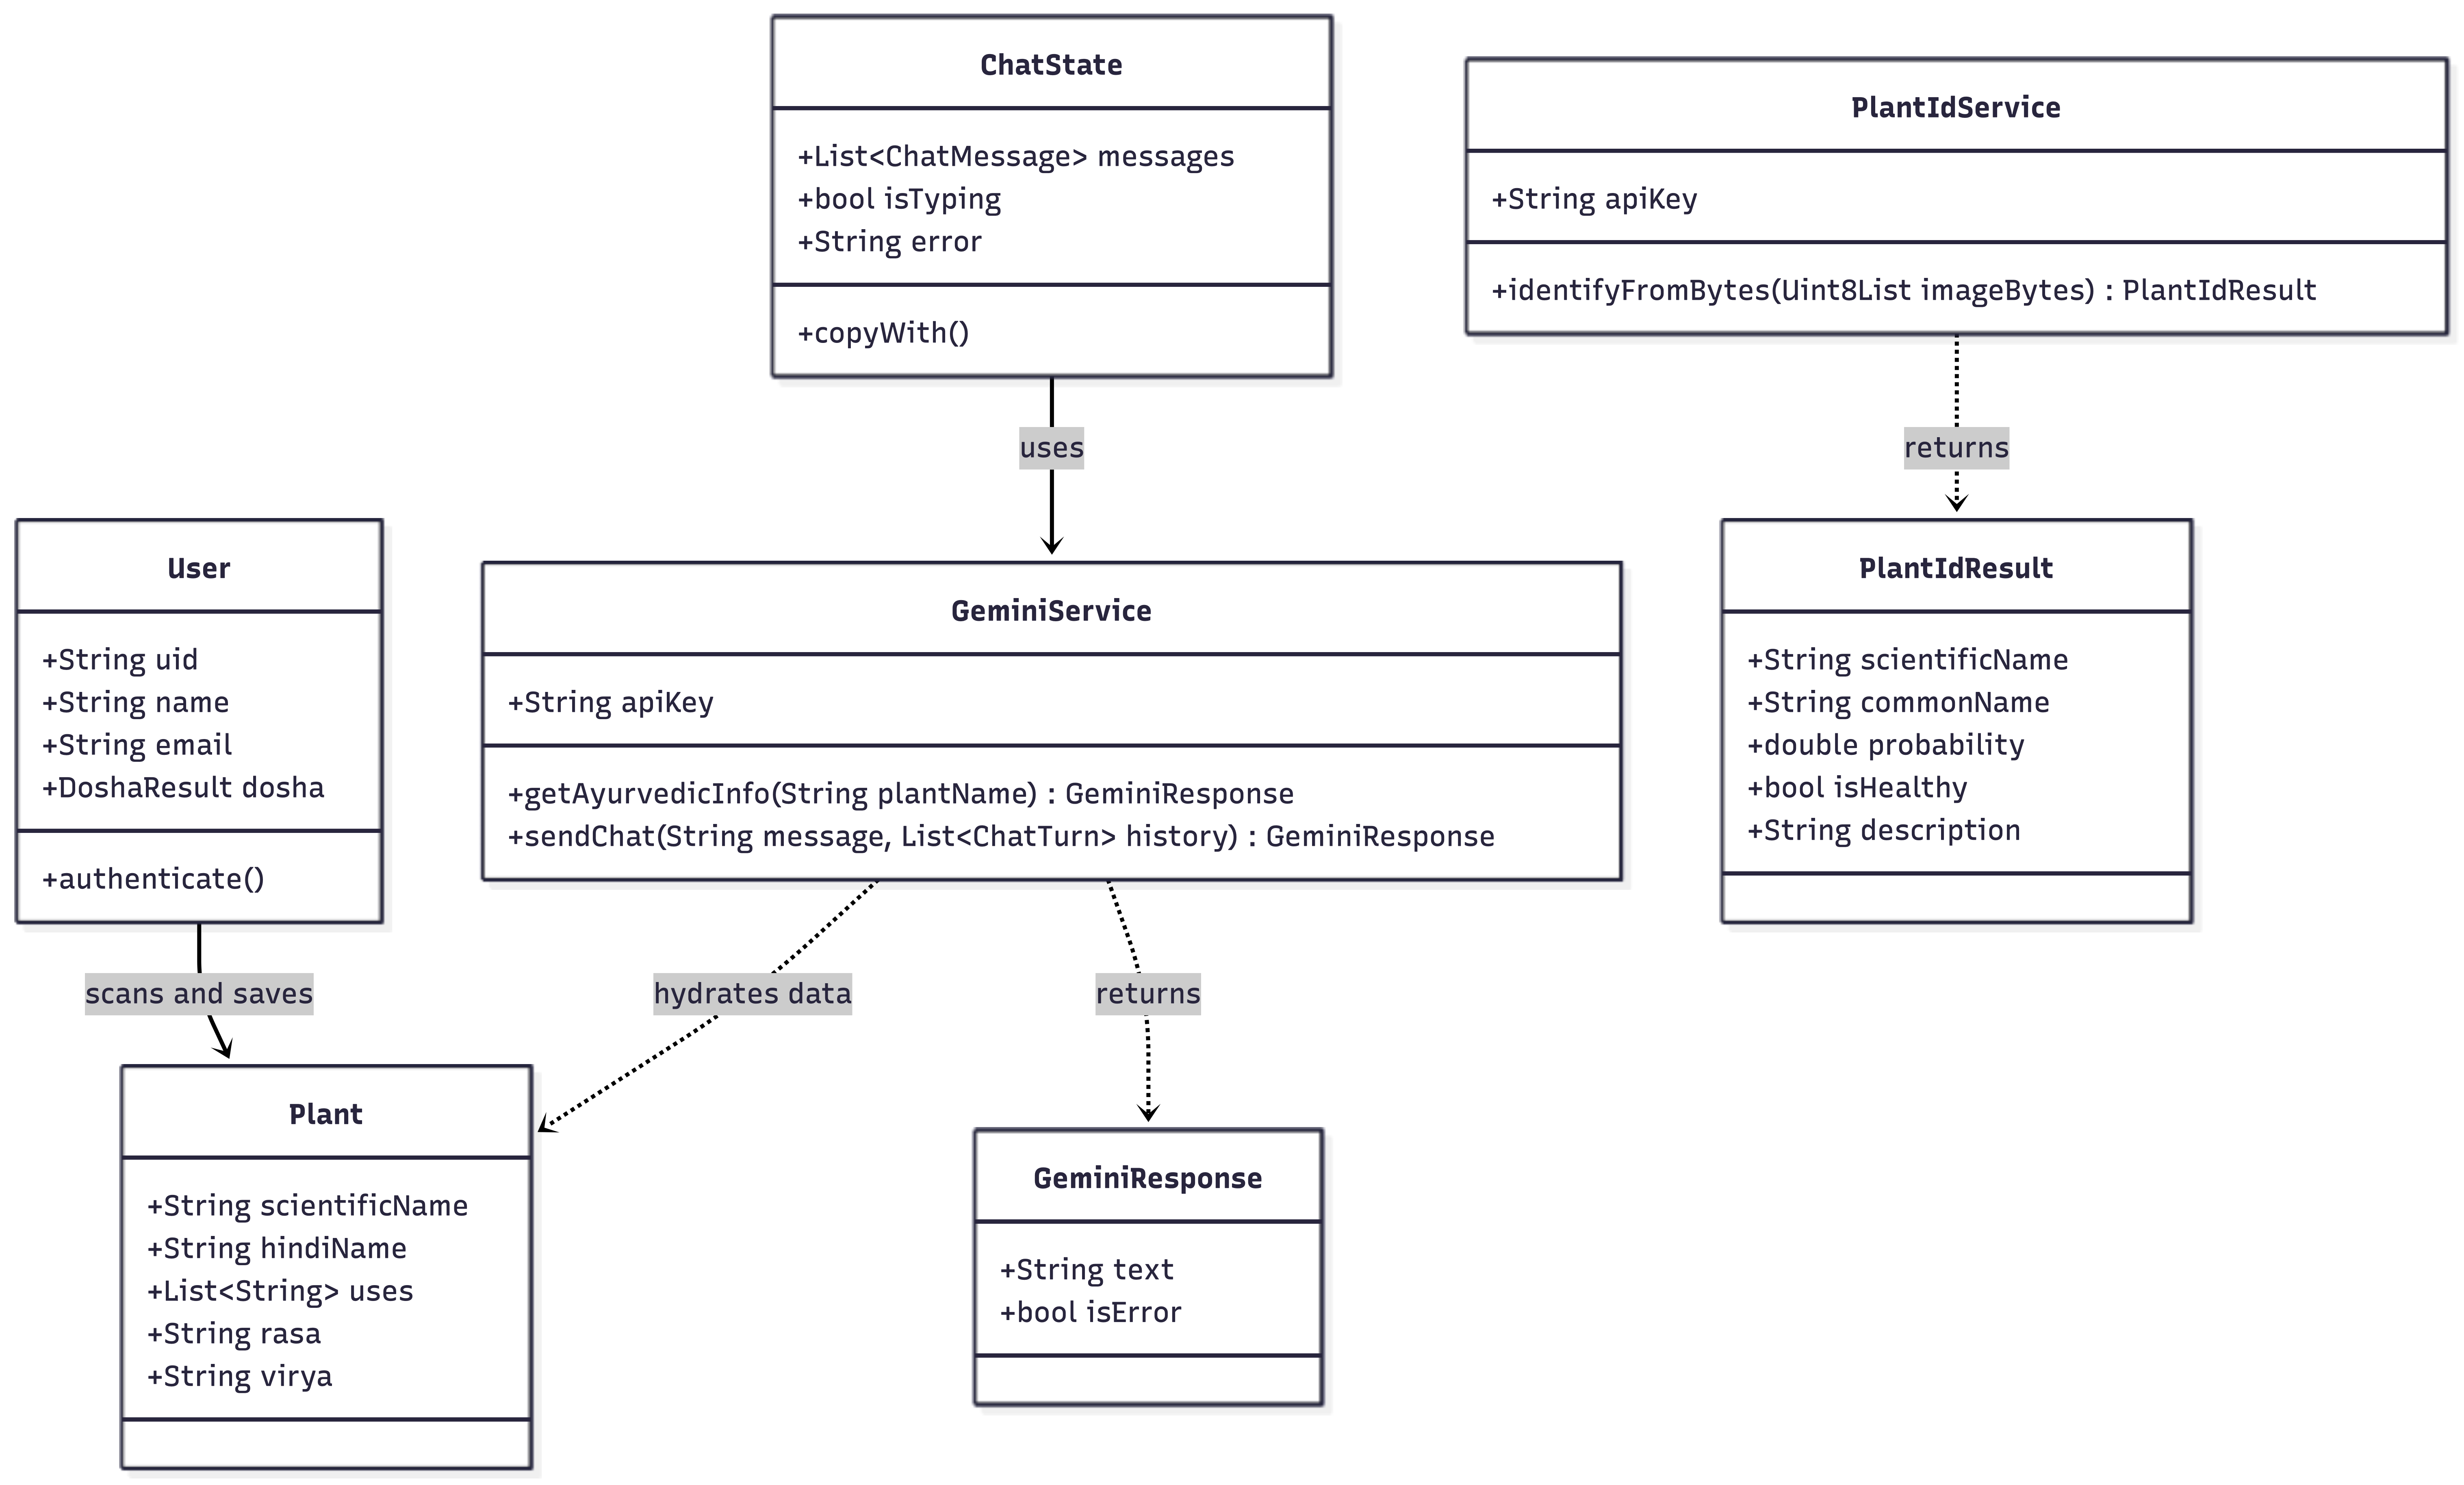
\includegraphics[width=0.91\linewidth,height=0.55\textheight]{placeholder_class_diagram.png}
  \end{mdframed}
    \caption{Class Diagram}
\end{figure}


\newpage
\section{Activity Diagram}
The activity diagram captures the procedural logic of the plant scanning and identification flow. It maps the user interaction starting from the Dashboard to the camera interface. After capturing an image, an internal processing phase compresses it. The data queries the Plant.id API. A critical confidence threshold gate triggers: if probability $< 0.2$, the user is shown an error/retry state. If successfully beyond $0.2$, it proceeds to query the Gemini API to formulate Ayurvedic interpretations, finally storing the data into Firestore and presenting it back to the user interface.

\renewcommand{\thefigure}{5.3}
\begin{figure}[!htpb]
\begin{mdframed}
    \centering
    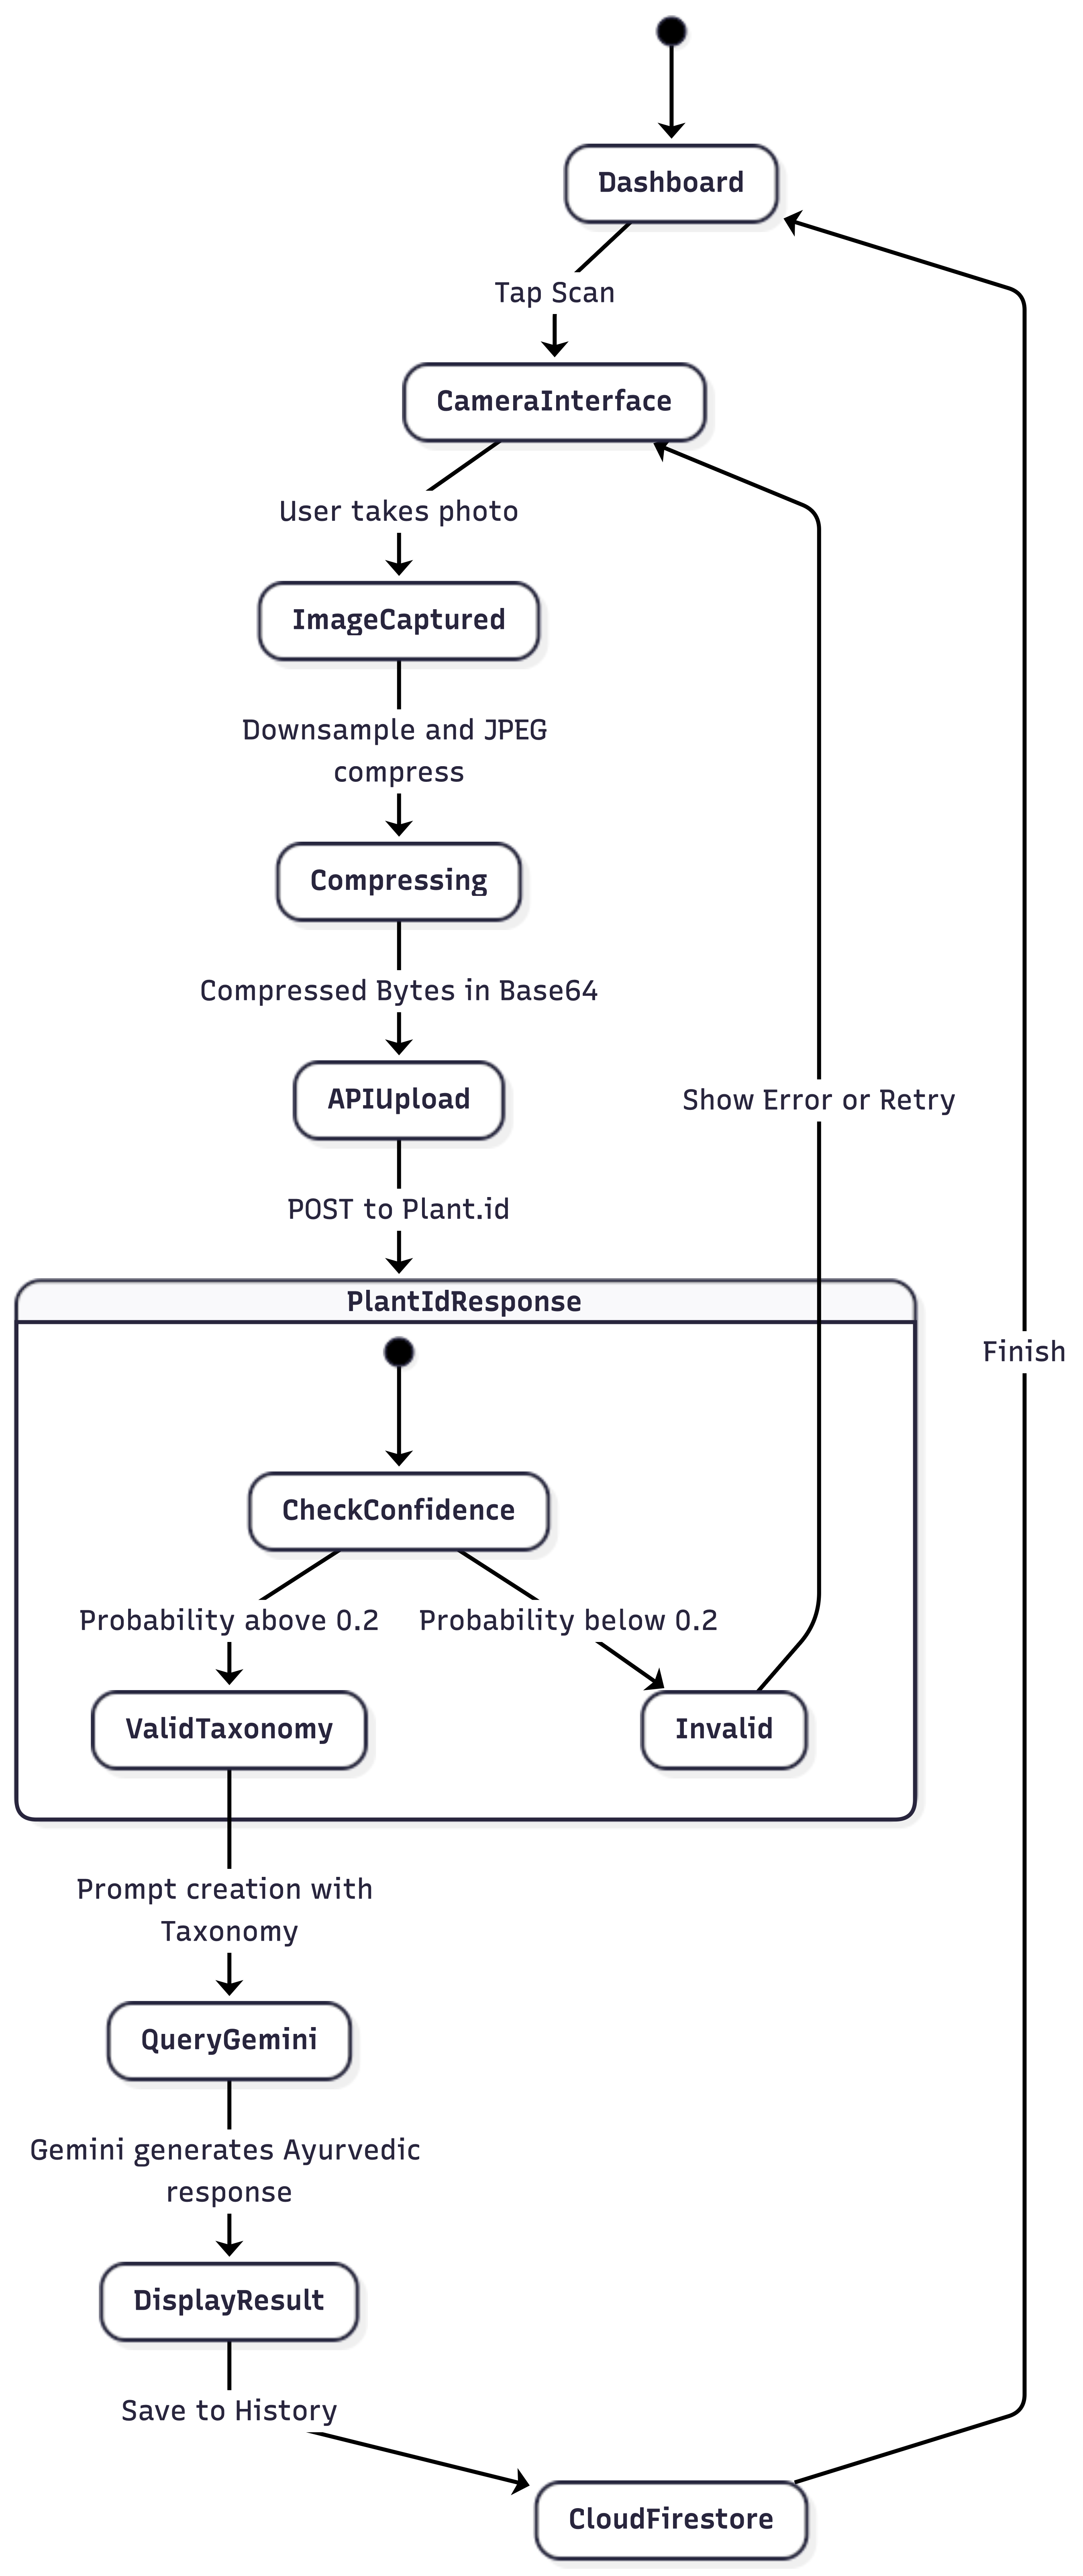
\includegraphics[width=0.5\linewidth,keepaspectratio]{placeholder_activity.png}
\end{mdframed}
    \caption{Activity Diagram}
\end{figure}


\newpage

\section{Sequence Diagram}
\justify
The Sequence Diagram outlines the timeline flow of execution. The user initiates an image upload via the Flutter Client. The client compresses the data and sends a POST request to the Plant.id engine. Based on success, the client takes the plant taxonomy return, constructs a Prompt incorporating this plant type, and transmits it via POST to the Gemini API layer. The generated comprehensive JSON properties are fetched. Finally, asynchronous calls record this event loop successfully to Cloud Firestore, updating the front-end dashboard for the Mobile User.

\vspace{2pt}
\renewcommand{\thefigure}{5.4}
\begin{figure}[!htpb]
\begin{mdframed}
     \centering
    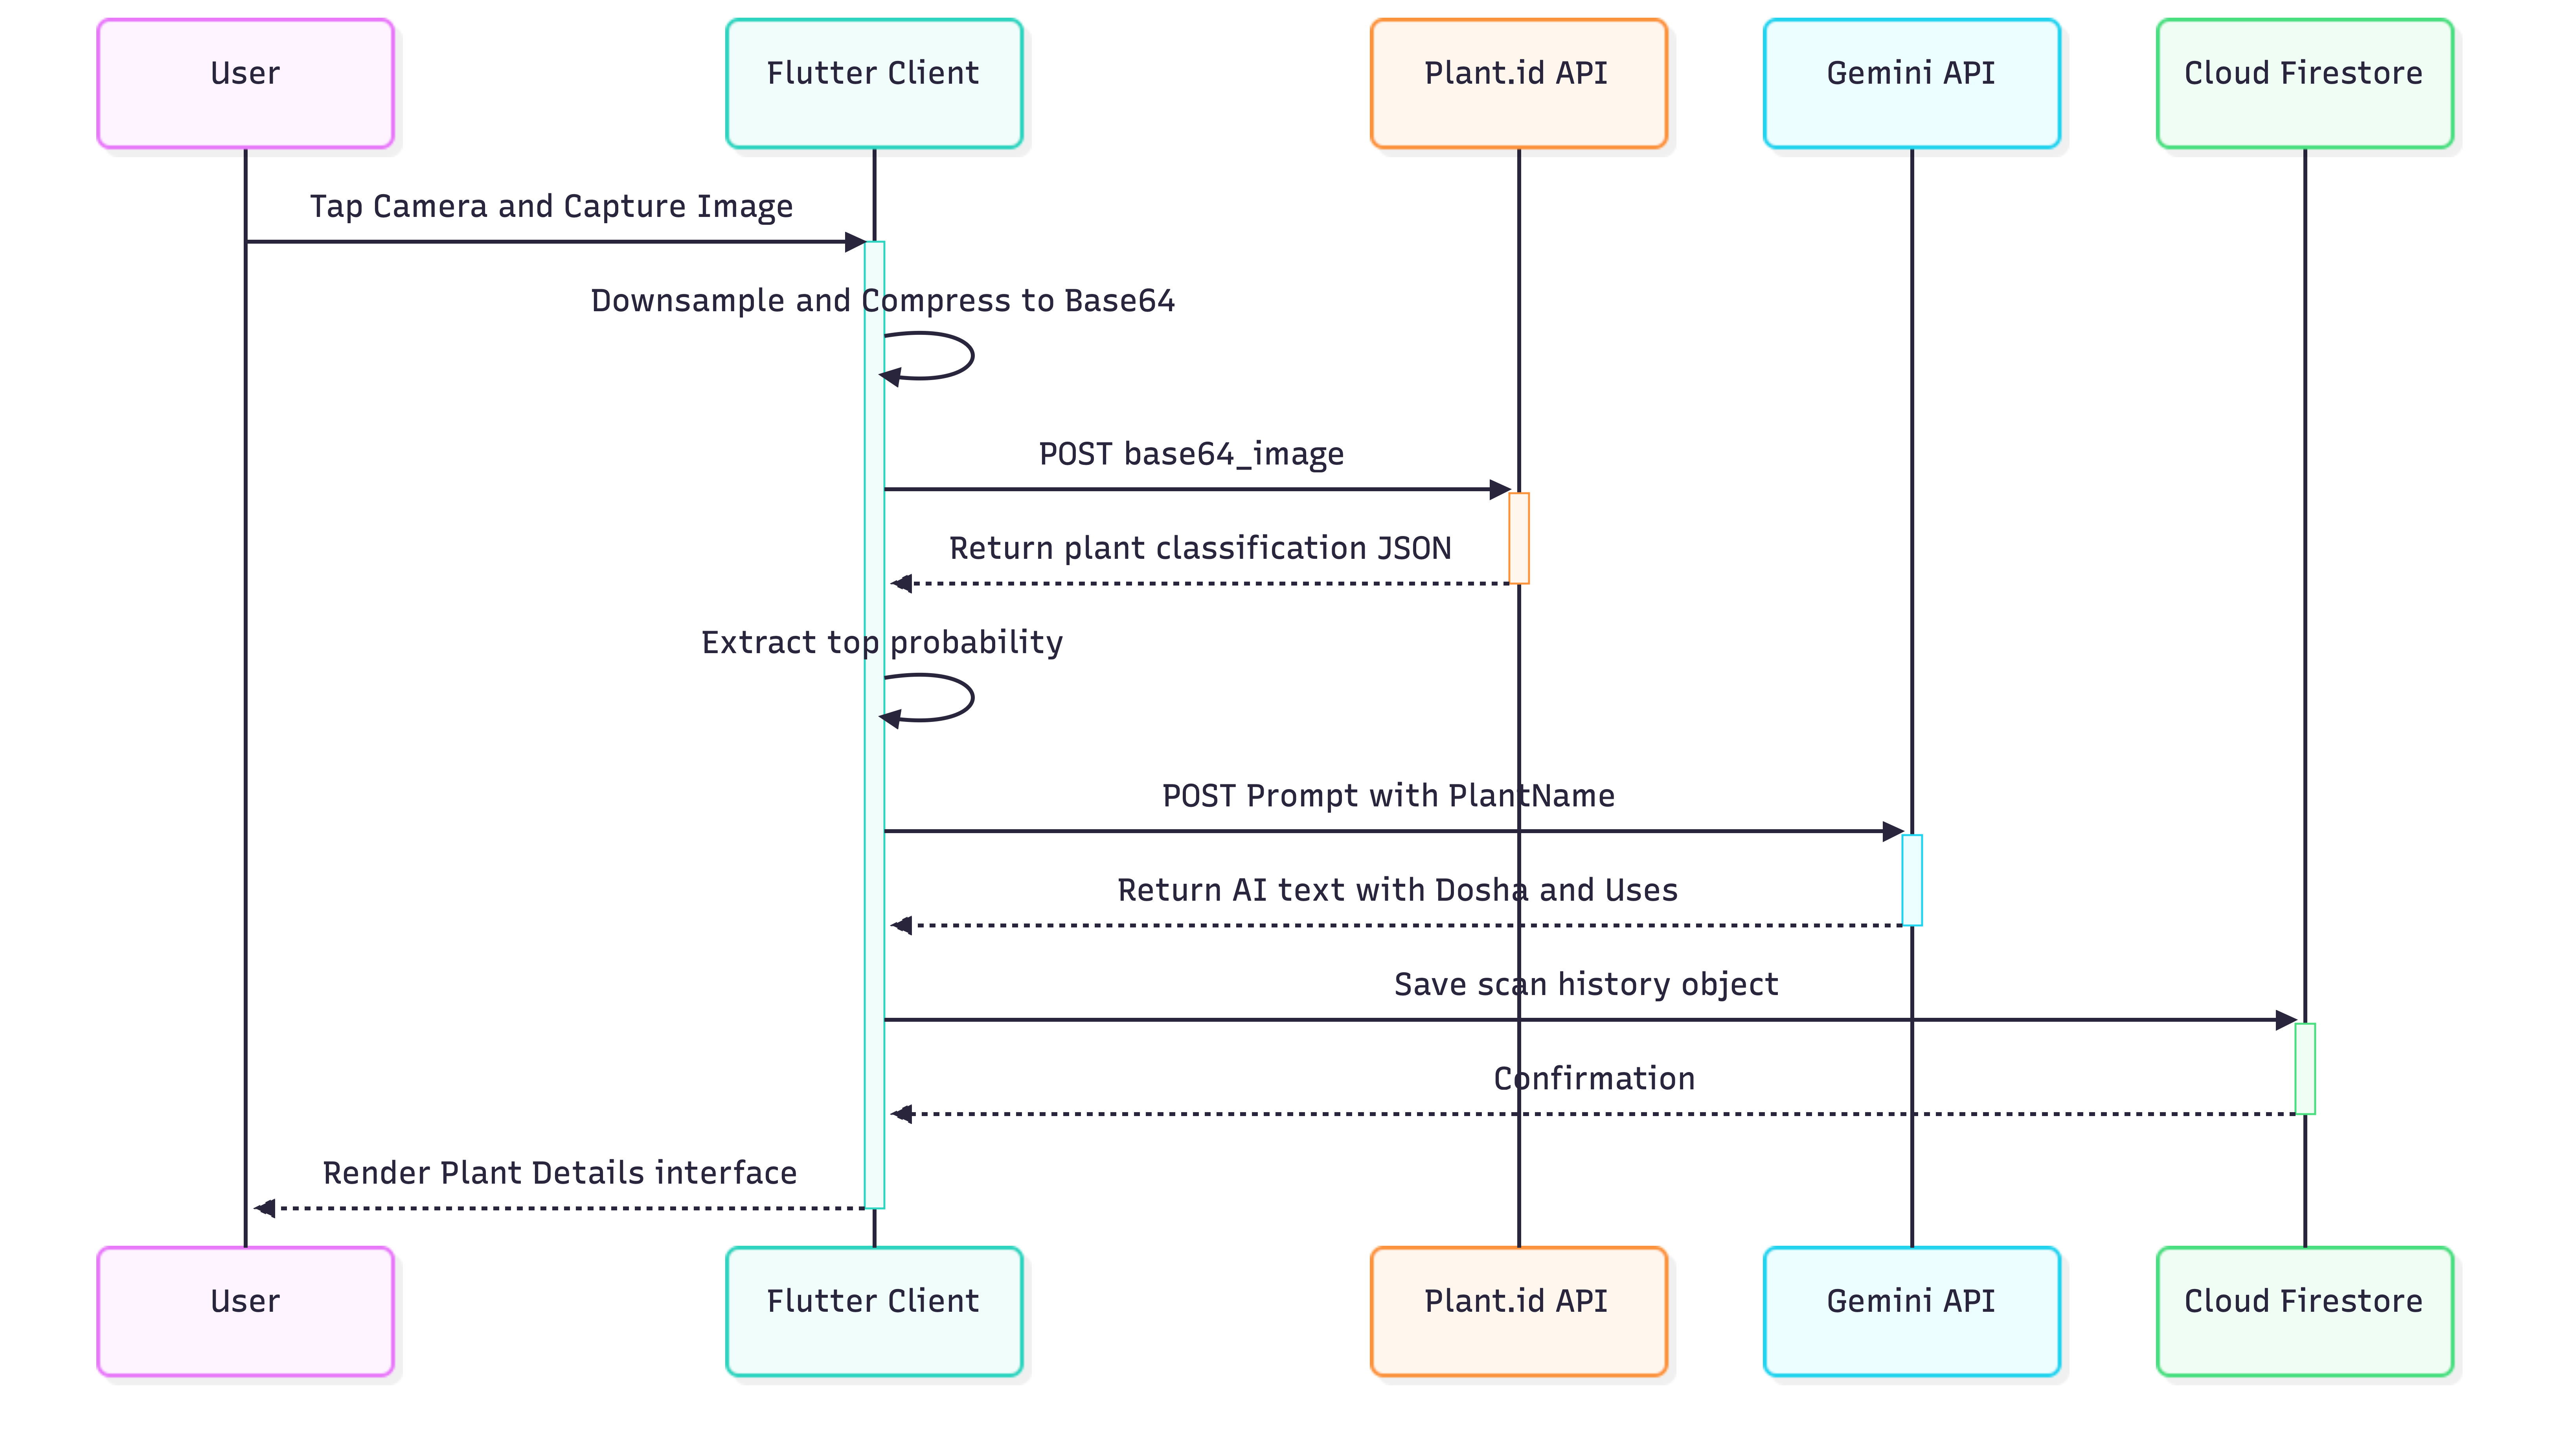
\includegraphics[width=0.84\linewidth,height=0.6\textheight]{placeholder_sequence.png}
\end{mdframed}
    \caption{Sequence Diagram}
\end{figure}
